\chapter{IntroductIon}

During the last few years, deep neural networks have gained considerable attention in several problems of computer vision.
The new network hierarchies present complex transfer modalities to deal with adaptive learning tasks.
Deep neural networks (DNN) allow machines to learn hybrid data structures of mathematical models which can be used to achieve comprehensive data analysis.
Image semantics would be resolved using relevant models.
The learning rate is measured in DNN by the achievement of comprehensive data analysis.
Generative adversarial networks (GANs) deal with a new hierarchy in intelligent systems.
The network scheme conforms to better training performance with less annotations.
GAN achievement is derived through a competitive learning where the model consists of different stacks.
The processing in layers is characterized with multiple levels of abstraction from high-dimensional input data.

In medicine, lesion detection becomes more efficient with new models based on deep learning networks from histological to radiological acquisitions.
Recent studies reveal that detection performance of deep networks has even matched or exceeded human-level performance in several tasks such as diabetic retinopathy and tumor detection \cite{gulshan2016development},\cite{icsin2016review}.
Early detection of cancer is considered as one the most complex and hard problems in radiology.
The follow-ups and repeated cases are also challenges for the correct decision making.
Over the last decade, the progress and the integration of DNN enable rapid diagnosis of patients at these risk groups.
Even if the final medical decision must be taken with a specialist, DNNs might reduce the time for the diagnostic errors and workload of physicians.
Therefore, DNN performance is not compared with physicians in our study.
The evaluation of DNN based segmentation is performed through Ground Truth; a mask which identifies the whole area or volume in target images.

The common goal of deep learning techniques is to recursively learn computational model parameters using a training dataset to gradually improve the model in performing the desired purpose.
Using many previously unseen data, models can also perform the same task accurately once a computer is trained for a specific task.
The strong generalization ability of deep learning now distinguish it from the other techniques of machine learning.
The detection and evaluation criteria result that the use of multilayered hierarchy of GAN shows valid scores.
The variation of inter observer, the inhomogeneity in image scale encompass the complexity of automatic lesion detection.
In skin lesion segmentation, International Skin Imaging Collaboration (ISIC) focuses on the analysis and the improvement of big datasets.
Annotated image corpora is considered as a challenge in deep learning for detection and classification.
Even if recent studies in data challenges promised valid results for clinical applications, the performance evaluation shows that training datasets might cause variation in skin lesion detection.
In order to promote automatic analysis in this field, GAN technique that represents promising scores is preferred.
Although many studies have been presented in this area, it can be seen that the success in the field of skin segmentation can be increased even further.
The International Skin Imaging Collaboration (ISIC) focused on automatic analysis of skin lesions, it has been trying to enrich the dataset regularly since 2016.
Annotated skin lesion images are presented in ISIC 2017 which can be used in feature extraction for automatic lesion segmentation tasks.

\begin{figure}
    \centerline{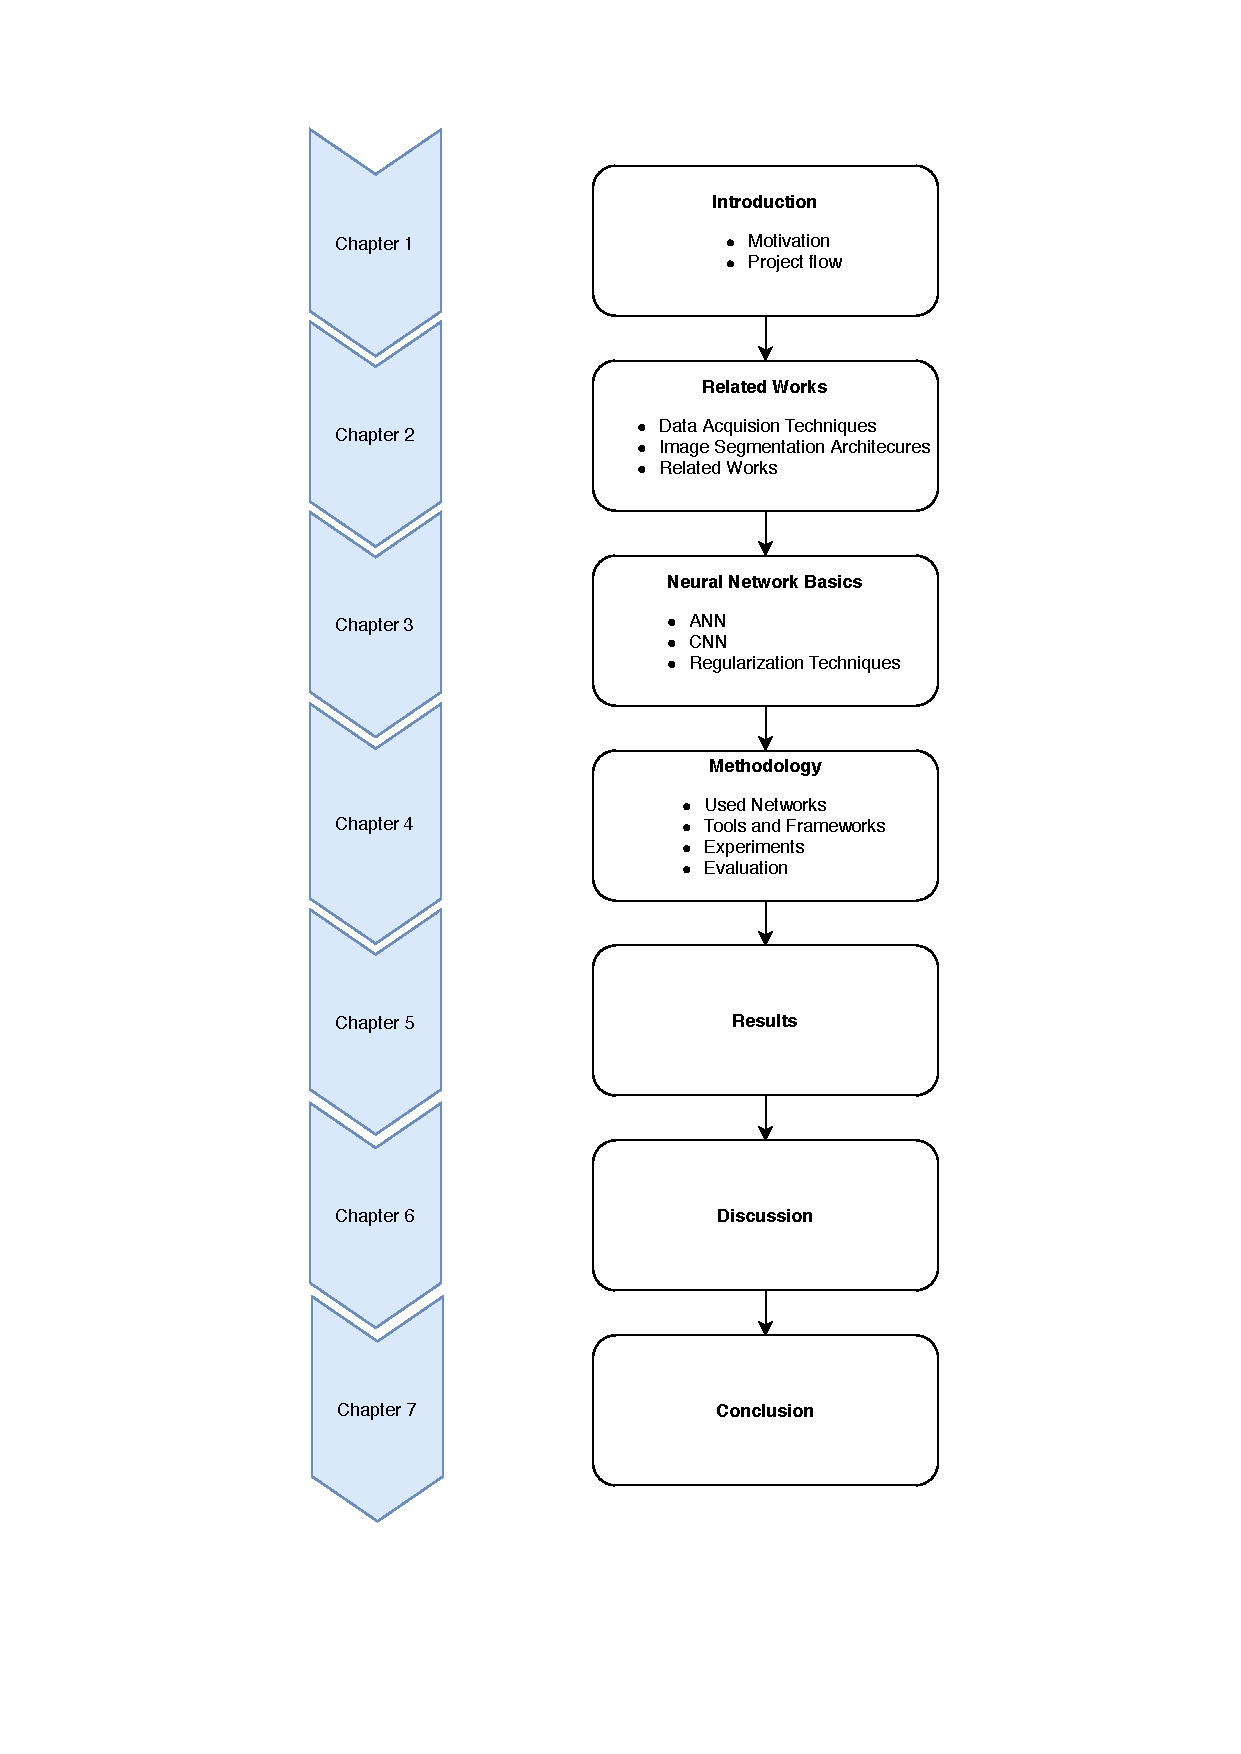
\includegraphics[width=1\columnwidth]{01-introduction/figures/project-flow.pdf}}
    \caption{ Thesis flow }
    \label{figure:project-flow}
\end{figure}

In this thesis, we provide a new application area of deep neural networks in skin lesion analysis.
We note that dermoscopic feature extraction is relatively a new problem in deep learning to address the detection and the classification of lesions.
The following section presents the medical imaging techniques, image segmentation architectures for automatic diagnosis of skin lesions from dermoscopic images and related studies of DNN for medicine.
The third section shows the basis of neural networks and convolutional neural networks.
Used neural network architectures, dataset, tools and deep learning frameworks are explained in fourth section
along with our corresponding formulation through computational parameters and the statistical evaluation.
Our detection results are given through statistical parameters in the fifth section.
Finally, the assessment of examined neural networks in skin lesion detection is concluded through the current state-of-the-art and prospective improvements. The project flow is summarized in Figure~\ref{fig:project-flow}.